\begin{figure}
	\[
		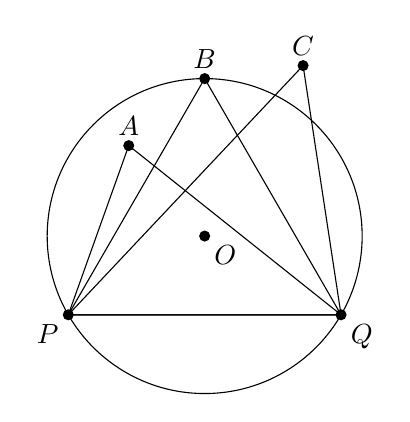
\begin{tikzpicture}[scale=2]
			% Draw the circle
			\draw (0,0) circle (1);

			% Define vertices (TikZ uses degrees)
			\coordinate (O) at (0:0);
			\coordinate (P) at (210:1);
			\coordinate (Q) at (330:1);

			\coordinate (A) at (130:.75);
			\coordinate (B) at (90:1);
			\coordinate (C) at (60:1.25);

			% Draw the triangle
			\draw (P) -- (Q) -- (B) -- cycle;
			\draw (P) -- (Q) -- (A) -- cycle;
			\draw (P) -- (Q) -- (C) -- cycle;

			% Optional: mark the vertices
			\fill (A) circle (1pt);
			\fill (B) circle (1pt);
			\fill (C) circle (1pt);
			\fill (P) circle (1pt);
			\fill (Q) circle (1pt);
			\fill (O) circle (1pt);

			% Labels
			\node[below right] at (O) {$O$};
			\node[below right] at (Q) {$Q$};
			\node[below left] at (P) {$P$};

			\node[above] at (A) {$A$};
			\node[above] at (B) {$B$};
			\node[above] at (C) {$C$};
		\end{tikzpicture}
	\]
	\caption{Three points with the same central angle inside, on, and outside the circle}
	\label{fig_thales}
\end{figure}
